\documentclass[12pt, a4paper, twoside, titlepage]{article}
%\usepackage[utf8]{inputenc}
%\usepackage[hungarian]{babel} %for hungarian language

\title{EFRP - Assignment 3}
\date{\today}
\author{Marcell Granát \\ Corvinus University of Budapest}

\usepackage{pdfpages}
\usepackage{graphicx}
\usepackage[hidelinks]{hyperref}
\usepackage{fancyhdr}

\pagestyle{fancy}
\fancyhf{}
\fancyhead[LE,RO]{Marcell Granát}
\fancyhead[RE,LO]{\leftmark}
\cfoot{\thepage}

\begin{document}
  \maketitle
  \tableofcontents
  
% --------------------------------------------------------  

\section*{Introduction}
\setcounter{page}{1}

This short paper is about an empirical analysis about cointegration using six stock prices (downloaded from Bloomberg) from 2003 December to 2019 June. Testing cointegration between stocks is a relevant technique to pairs trading, which is a widely used strategy. However pairs trading may be based on several pairs choosing rules, many papers concluded formerly, that cointegration leads to higher profitability on real world data
%\cite{Huck.2014}.
In this study I do not focus on this methods efficiency, only on the frequency of cointegrated stock prices. For this purpose I commit two different cointegration-test (Engel-Granger method and Johansen test) on the full time-interval, after I also use this methods with rolling windows. All the R codes of this paper are uploaded to my public github repository (\href{https://github.com/MarcellGranat/EFRP/blob/master/Exercise-3.md}{https://github.com/MarcellGranat/EFRP}). 

\section*{Engle-Granger method}

Engle-Granger method is simple way to test cointegration in bivariate case. Cointegration is diagnosed if the two tested series are integrated in the same order and a linear combination of them exist, which has an integration order of the original non-stationer series minus one %\cite{Kirchgassner.2007}.
The most common is when the tested stock prices are I(1) and their linear combination is stationer.

The used stock prices are presented in figure \ref{fig1}. For a first glance there is a high chance that some cointegrated pairs can be found in this set of series. To commit the tests the first step is to check the time-series integration order. For this purpose I use ADF-test with a significance level 5\%. As a result it is concluded that all the series are I(1), if any of their bivariate linear combination is stationer, then cointegration is diagnosed. The first difference of the stock prices is shown on figure \ref{fig3}.

The second step is run OLS with all the possible pairs and check if there is a series of residuals stationer. Just as at the previous step the stationary test is augmented Dickey-Fuller test without constant or trend component in the auxiliary regression and $\alpha = 5\%$.

With the described parameters \footnote{In my previously mentioned github repository you may find that I wrote an R function to commit the whole Engle-Granger method with specified parameters. It would be reasonable to see the results with different stationary test or with different significance level (specially if calculating its profitability is also in focus). With the written function, it is possible to modify the test parameters and see how the results change.} the tests confirms only one cointegrated pair (see Figure \ref{fig4}), and that result holds only if the stock price of Bank of America is in regressor role, but is does not, when that is used as dependent variable\footnote{The matrix of the results is not a symmetrical.}.

\section*{Johansen test}

Johansen test is adequate cointegration test, when there are more that two tested series at the same time. This test is performed in order to estimate the number of cointegrated vectors (r) in the system. If there is any cointegration in the model then $0<r<k$, where k is number of tested time-series. The system decomposition is not unique, so we can only estimate the cointegration rank r %\cite{Kirchgassner.2007}.
The method can be performed with several tests, in this paper I chose the Lmax test. It gives a vector of test statistic as a result and that may be compared to critical values. The null hypothesis is that $r \leq x$, where $x = 0, 1, 2, ..., k-1$. The number of cointegrated vectors is the smallest $x$, under which null hyphothesis is not rejected. The empirical analysis in this study shows that the r in this system is 1 on the full time-interval\footnote{Same result is stated on 1\%, 5\% and 10\% significance level.}, which confirms the identical result as the one found with the Engel-Granger method.

\section*{Engle-Granger method with rolling window}

In this section I expound the results of the previously presented Engle-Granger method performed with rolling windows. The size of windows is 250 days. Important to note, it is not sure that a stock price has the same integration order in each window. It can happen that a cointegration test is not permittable, because in that period the integration orders do not match. Since this calculation is realy time-consuming, only three of the six stock will be tested in this paper. This means that the maximum number of cointegrated pairs is 6 ($3 \times 3 - 3$). The test parameters are the same as described before, results are shown on figure \ref{fig6}.

In figure \ref{fig6} it can be seen that the number of cointegrated pairings reaches the maximum number at the end of 2008, 2012 and in the middle of 2008, 2016. In 2008 there is also a long preriod, when there are 4 cointegrated pairings. This result suggests a pattern that in recession cointegration may be more frequent.

\section*{Johansen-test with rolling window}



\begin{figure}[ht]
  \centering
  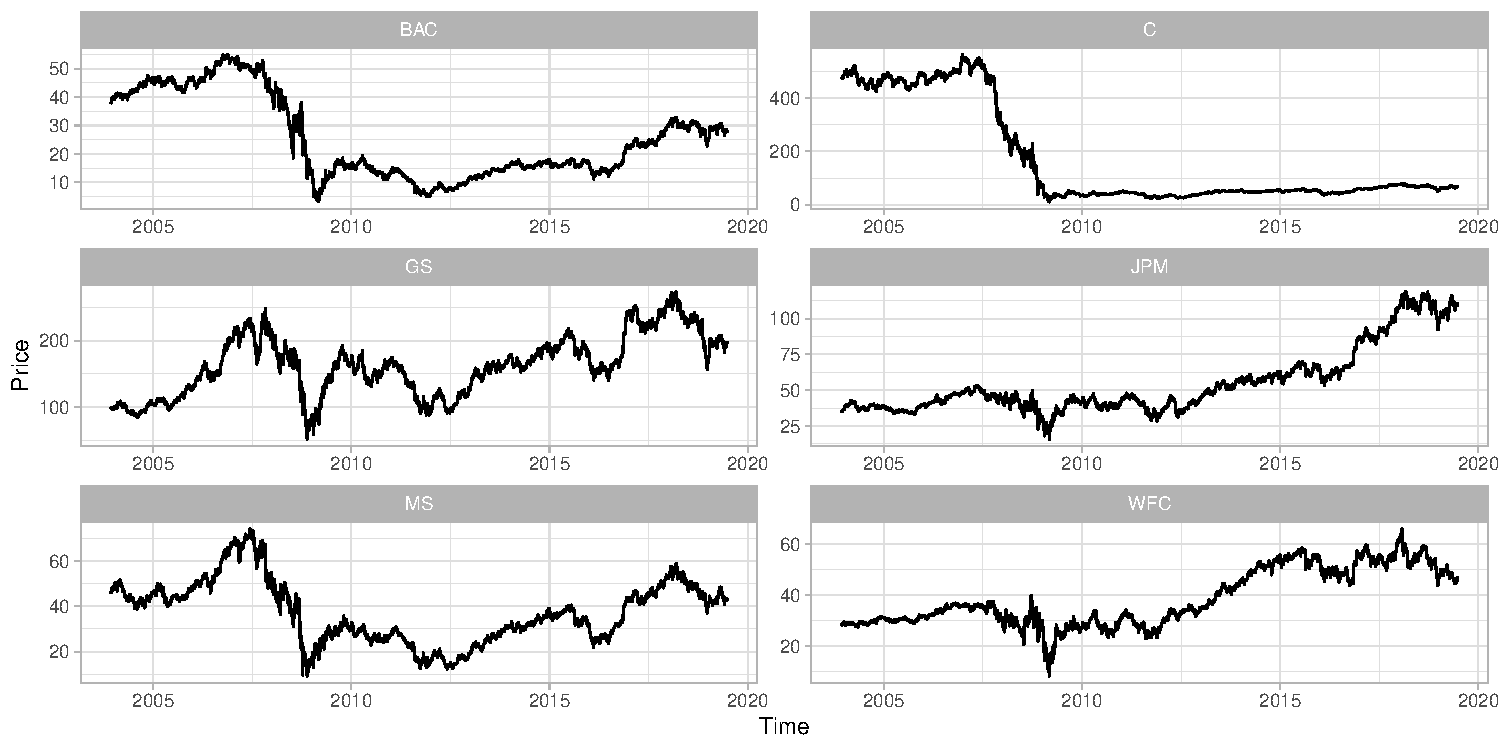
\includegraphics[width=\textwidth]{C:/rproject/EFRP/plot/unnamed-chunk-5-1.pdf}
  \caption{Time-series used in this study.}
  \label{fig1}
\end{figure}

\begin{figure}[ht]
  \centering
  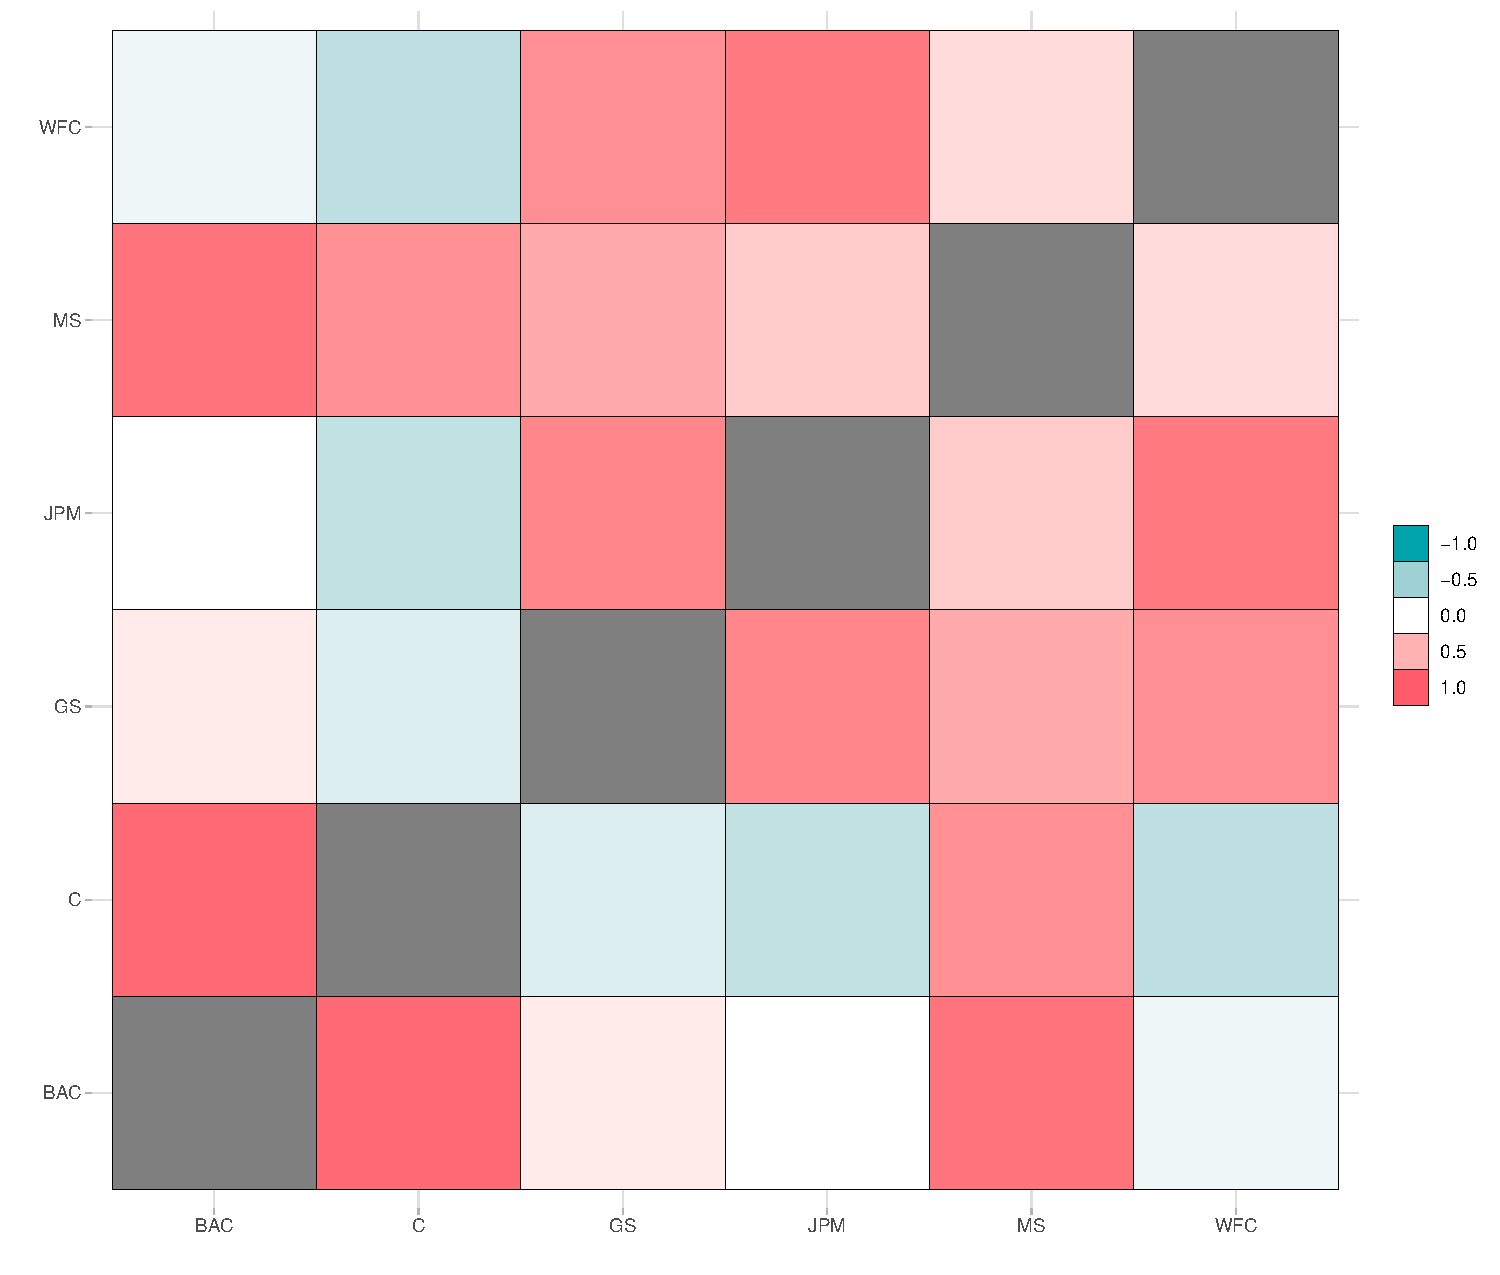
\includegraphics[width=\textwidth]{C:/rproject/EFRP/plot/unnamed-chunk-6-1.pdf}
  \caption{Correlation-matrix.}
  \label{fig2}
\end{figure}

\begin{figure}[ht]
  \centering
  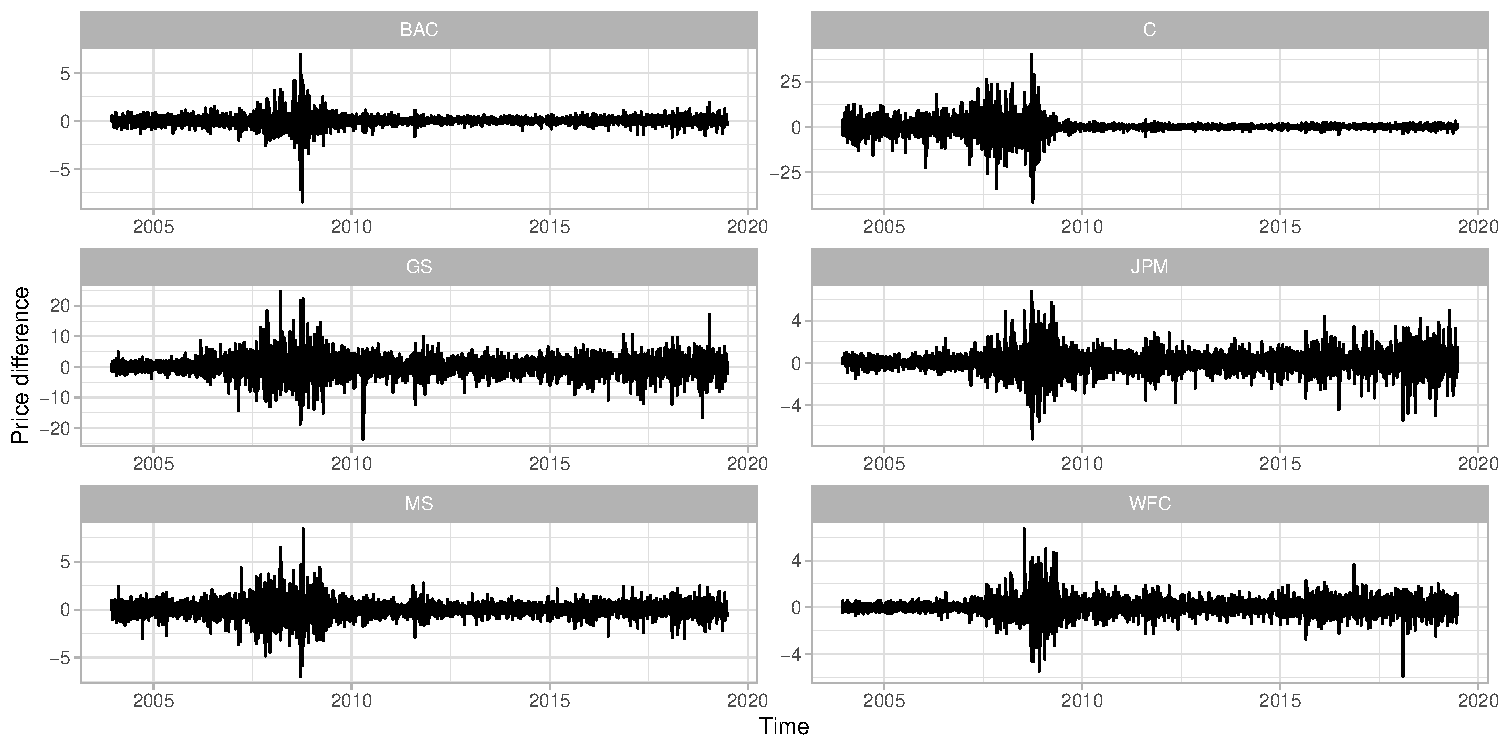
\includegraphics[width=\textwidth]{C:/rproject/EFRP/plot/unnamed-chunk-8-1.pdf}
  \caption{First difference of the time-series.}
  \label{fig3}
\end{figure}

\begin{figure}[ht]
  \centering
  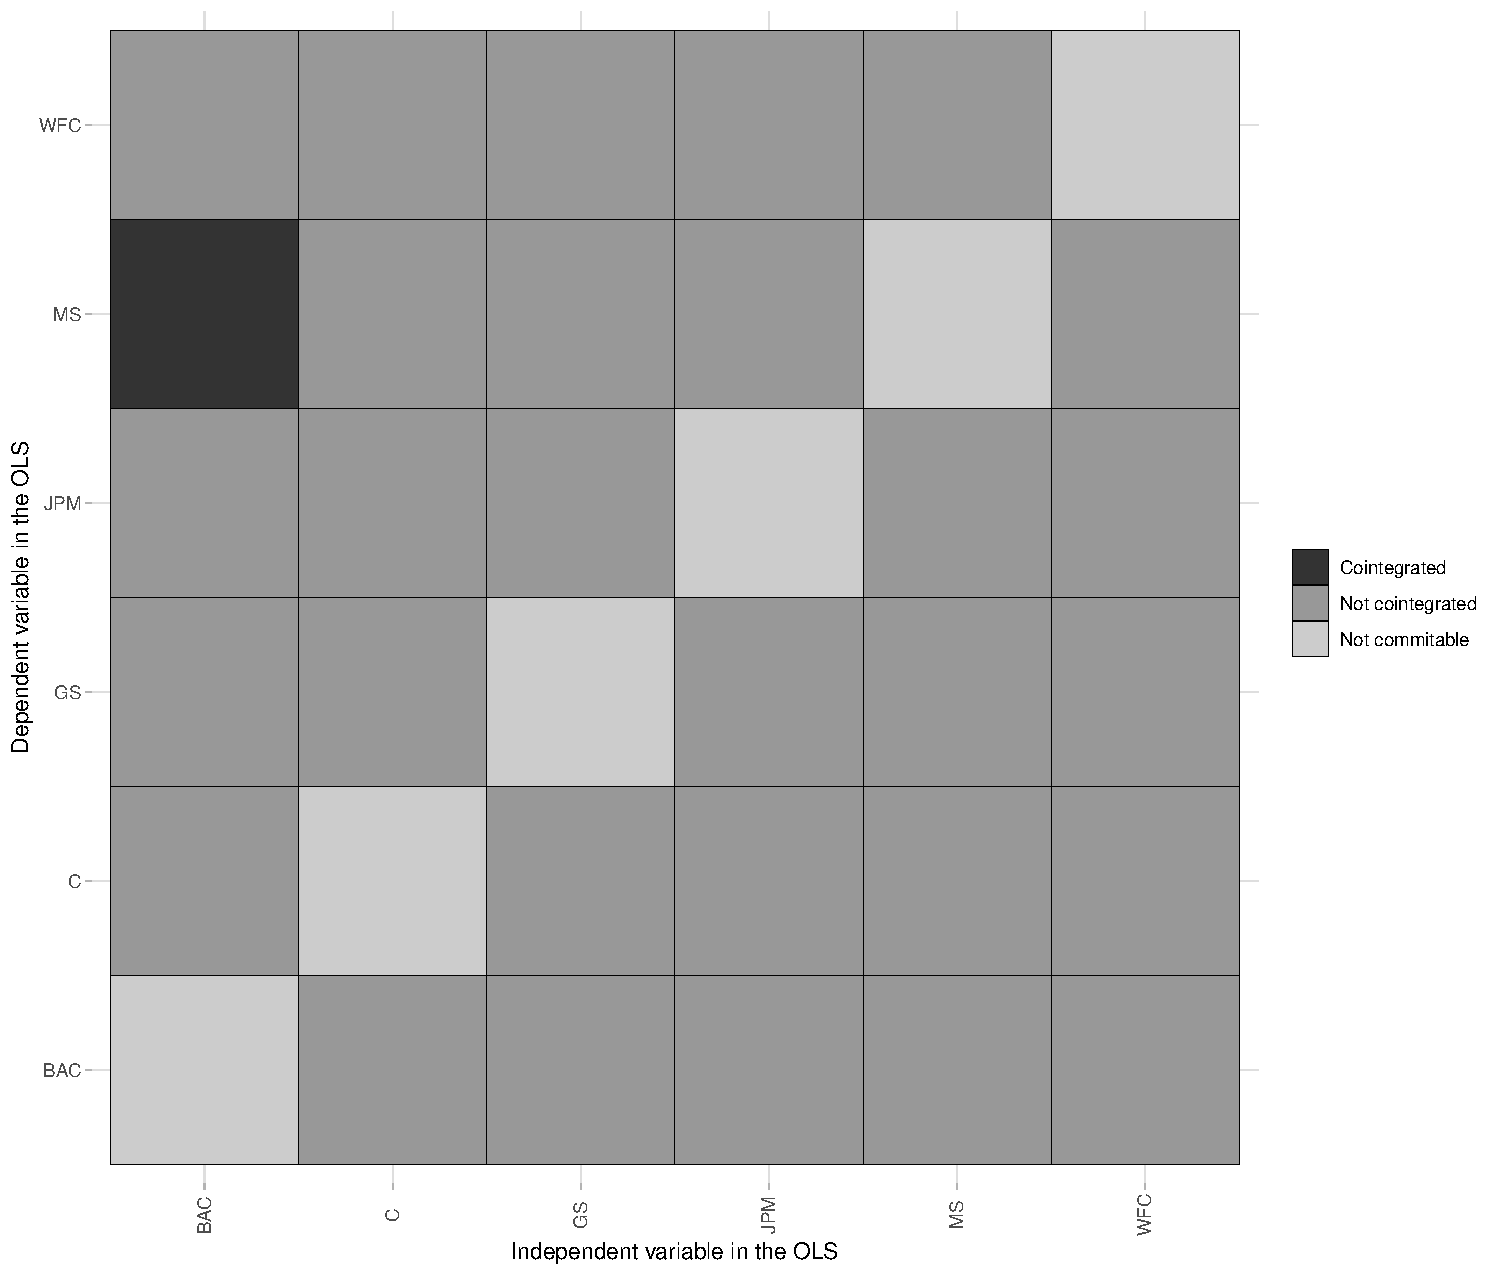
\includegraphics[width=\textwidth]{C:/rproject/EFRP/plot/unnamed-chunk-10-1.pdf}
  \caption{Results of Engle-Granger method.}
  \label{fig4}
  Calculations are based on ADF-test (level, $\alpha = 5\%$)
\end{figure}

\begin{figure}[ht]
  \centering
  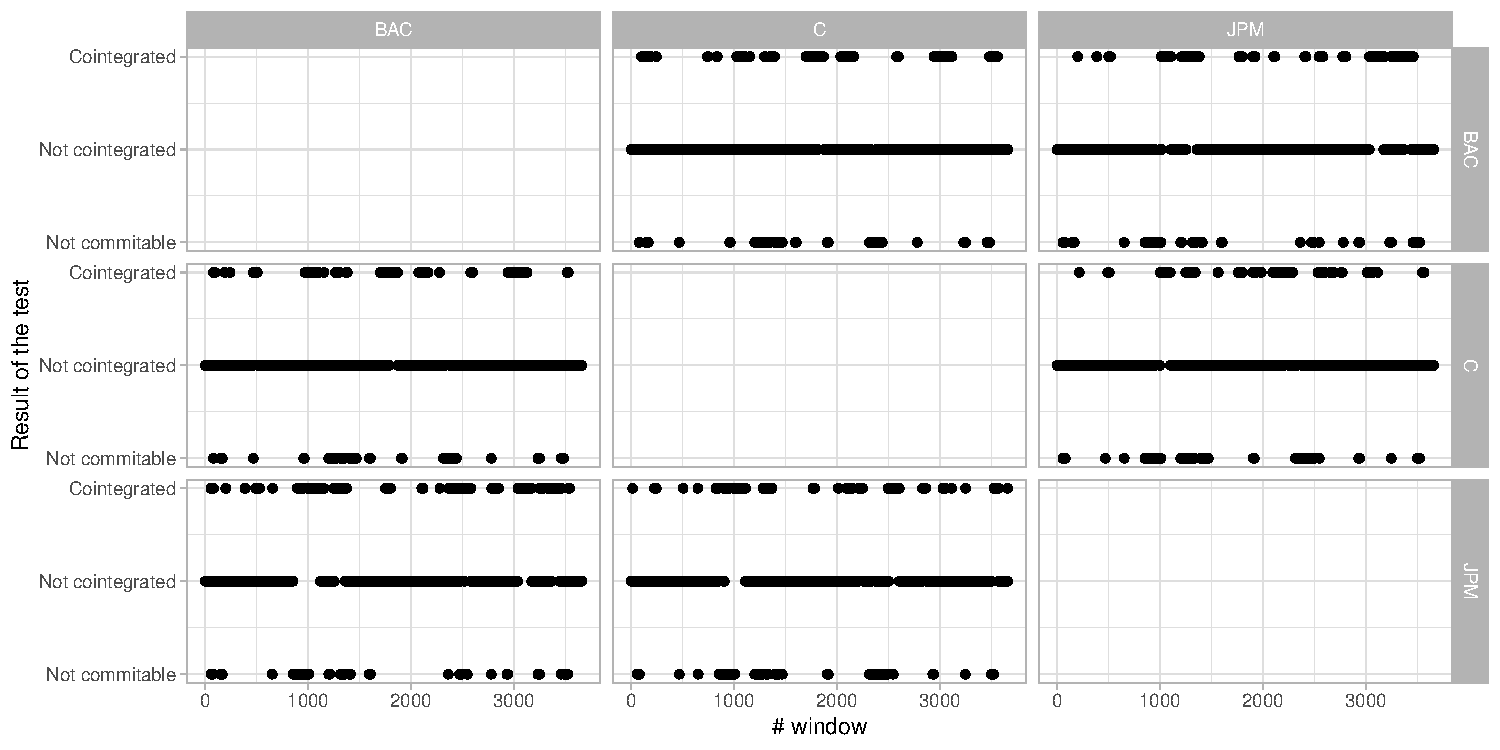
\includegraphics[width=\textwidth]{C:/rproject/EFRP/plot/unnamed-chunk-12-1.pdf}
  \caption{Results of Engle-Granger method with rolling window.}
  \label{fig5}
  Size of windows is 250 days. Calculations are based on ADF-test (level, $\alpha = 5\%$). Depedent variables (in the OLS) are placed horizontal, independents are vertical.
\end{figure}

\begin{figure}[ht]
  \centering
  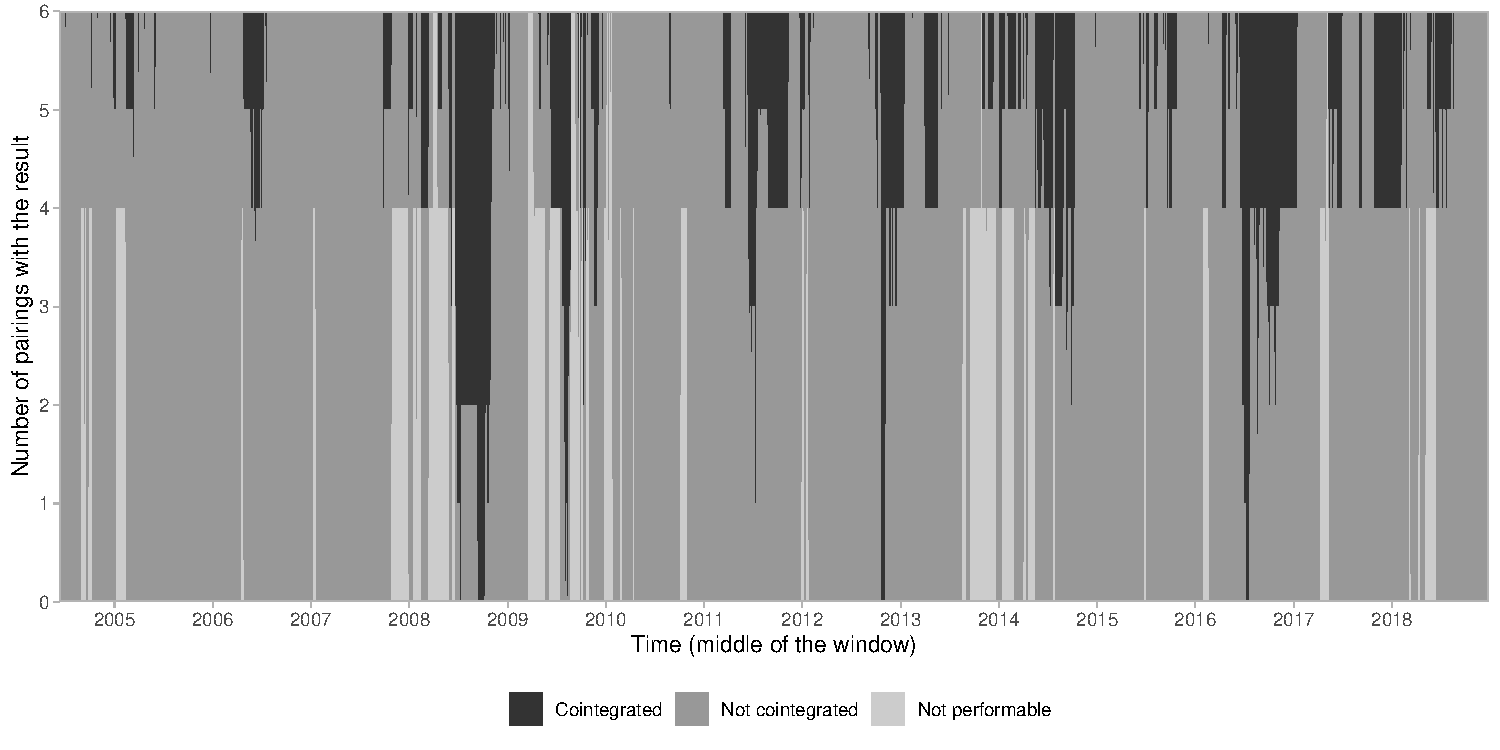
\includegraphics[width=\textwidth]{C:/rproject/EFRP/plot/unnamed-chunk-14-1.pdf}
  \caption{Summary results of Engle-Granger method with rolling window.}
  \label{fig6}
  Calculations are based on ADF-test (level, $\alpha = 5\%$). Number of total pairs is 6.
\end{figure}

\begin{figure}[ht]
  \centering
  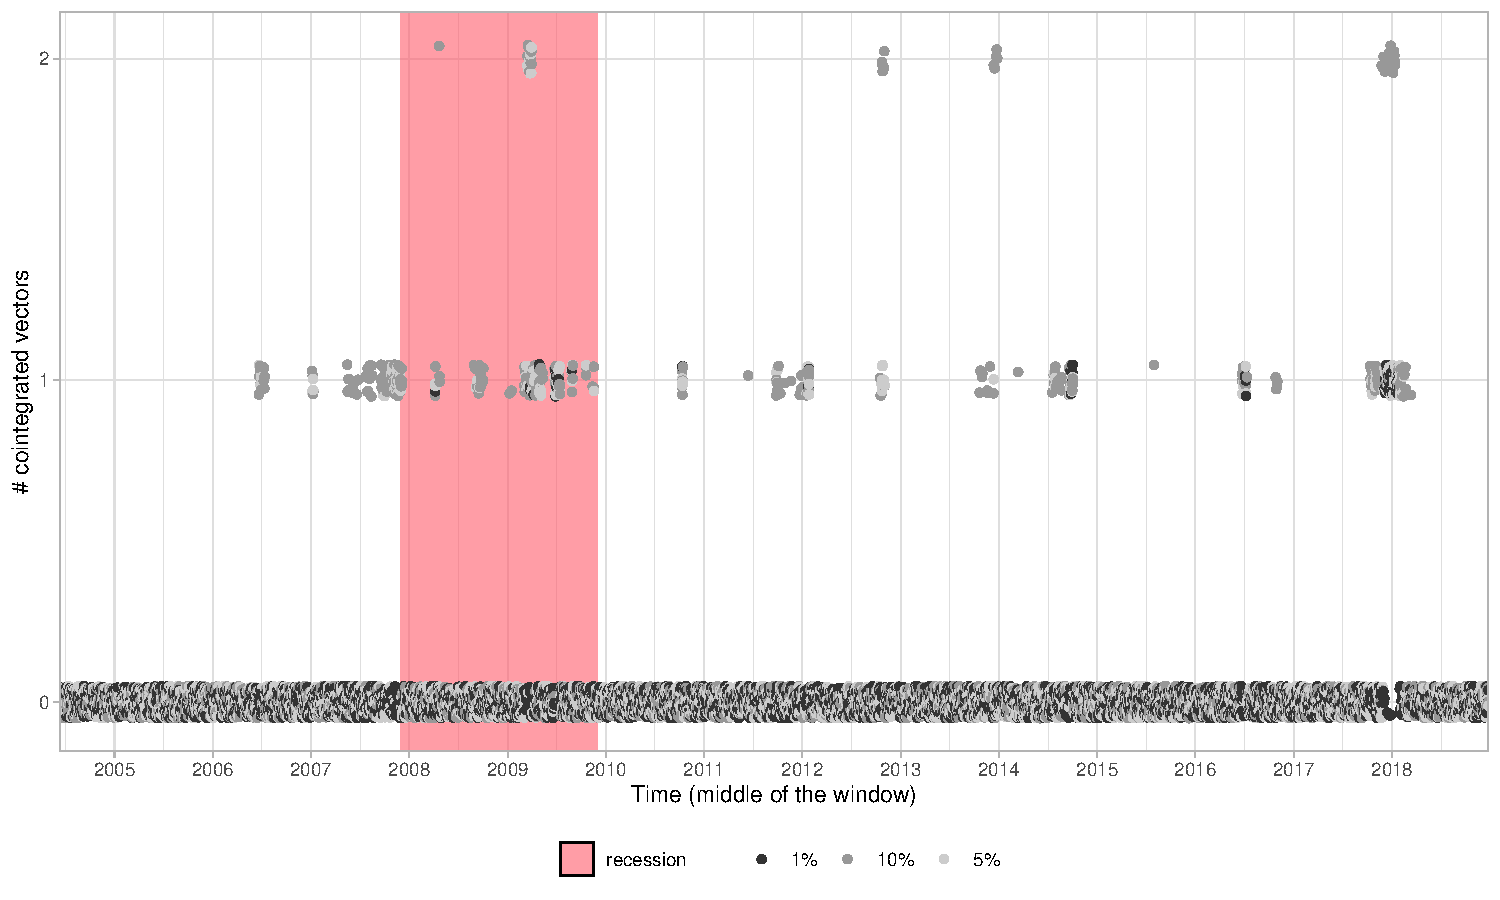
\includegraphics[width=\textwidth]{C:/rproject/EFRP/plot/unnamed-chunk-15-1.pdf}
  \caption{Results of Johansen test with rolling window across time.}
  \label{fig7}
  Size of windows is 250 days. Points are jittered around their true y value for better visualisation (the number of cointegrated vectors is interger). Date of recession is from the National Bureau of Economic Research (https://www.nber.org/cycles.html).
\end{figure}

\begin{figure}[ht]
  \centering
  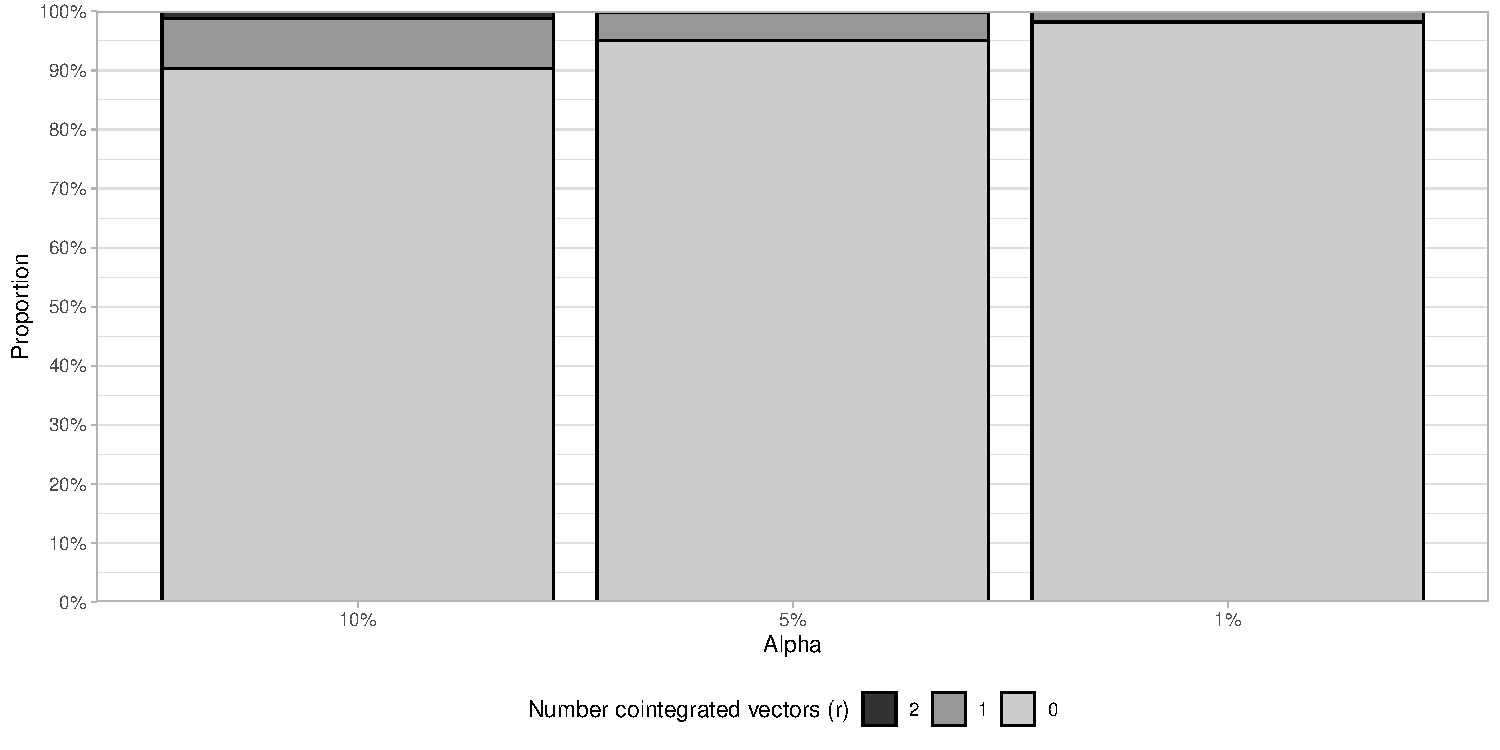
\includegraphics[width=\textwidth]{C:/rproject/EFRP/plot/unnamed-chunk-16-1.pdf}
  \caption{Distribution of the Johansen test results with rolling window.}
  \label{fig8}
\end{figure}

\begin{appendix}
  \listoffigures
  \listoftables
\end{appendix}

\bibliography{CointegrationBib}
\bibliographystyle{Apalike}

\end{document}